\documentclass[a4paper,12pt]{article}
\usepackage[utf8]{inputenc}
\usepackage[top=2cm,bottom=2.54cm,left=2.54cm,right=2.54cm]{geometry}
\usepackage[namelimits]{amsmath} 
\usepackage{amssymb}             
\usepackage{amsfonts}            
\usepackage{mathrsfs}            
\usepackage{graphicx}
\usepackage{subfigure}
\usepackage{multirow}
\usepackage{listings}
\usepackage{diagbox}
\usepackage{slashbox}
\lstset{language=Matlab}
\lstset{breaklines}
\lstset{extendedchars=false}

\title{Fintech545 Homework 3}
\author{qw112 Qiyu Wu}
\date{}

\begin{document}
\maketitle
\subsection*{Question 1. Expectation and Standard Deviation about Price}
For the problemset 1, we assume that $r_{t}\sim N(0,\sigma^2)$. We only concern the specific time t and t-1 period.
Therefore, for each method, our calculation will be based on a conditional probability density function $f(P_{t}|P_{t-1})$.

\subsubsection*{Classical Brownian Motion}
\begin{displaymath}
    \begin{split}
        P_t &= P_{t-1} + r_{t} \quad r_{t}\sim N(0,\sigma^2)\\
        E(P_t|P_{t-1}) &= E(P_{t-1}+r_{t}|P_{t-1}) = \int (P_{t-1}+r_{t})f(r_{t})dr_{t} = P_{t-1} + \int r_{t}f(r_{t})dr_{t} = P_{t-1}\\
        Var(P_t|P_{t-1}) &= Var(P_{t-1}+r_{t}|P_{t-1}) = E_{p_{t-1}}(P_{t-1}+r_{t}-E_{p_{t-1}}(P_{t-1}+r_{t}))^{2} = E(r_{t})^2 = \sigma^{2}\\
        Std(P_t|P_{t-1}) &= \sigma
    \end{split}
\end{displaymath}

\subsubsection*{Arithmetic Return System}
\begin{displaymath}
    \begin{split}
        P_t &= P_{t-1}(1+r_{t}) r_{t} \sim N(0,\sigma^2)\\
        E(P_t|P_{t-1}) &= E(P_{t-1}+P_{t-1}r_{t}|P_{t-1})=  \int (P_{t-1}(1+r_{t}))f(r_{t})dr_{t} = P_{t-1}+P_{t-1}\int r_{t}f(r_{t})dr_{t} = P_{t-1}\\
        Var(P_t|P_{t-1}) &= Var(P_{t-1}+P_{t-1}r_{t}|P_{t-1}) = E_{p_{t-1}}(P_{t-1}+P_{t-1}r_{t}-P_{t-1})^{2} = E_{p_{t-1}}(P_{t-1}r_{t})^2\\
         &= P_{t-1}^{2}E(r_{t})^{2} = P_{t-1}^{2}\sigma^{2}\\
        Std(P_t|P_{t-1}) &= P_{t-1}\sigma
    \end{split}
\end{displaymath}


\subsubsection*{Geometric Brownian Motion}
\begin{displaymath}
    \begin{split}
        P_{t} &= P_{t-1}e^{r_{t}}\\
        E(P_{t}|P_{t-1}) &= E(P_{t-1}e^{r_{t}}|P_{t-1}) = \int (P_{t-1}e^{r_{t}})f(r_{t})dr_{t} = P_{t-1}\int e^{r_{t}}f(r_{t})dr_{t} = P_{t-1}E(e^{r_{t}}) \\
                        & = P_{t-1} e^{\frac{\sigma^{2}}{2}}\\
        Var(P_t|P_{t-1}) &= Var(P_{t-1}e^{r_{t}}|P_{t-1}) = E_{p_{t-1}}(P_{t-1}e^{r_{t}}-E_{p_{t-1}}(P_{t-1}e^{r_{t}}))^{2}\\
                        &= P_{t-1}^{2}E(e^{r_{t}}-e^{\frac{\sigma^{2}}{2}})^{2} = P_{t-1}^{2}E(e^{2r_t}-2e^{r_t}e^{\frac{\sigma^{2}}{2}}+e^{\sigma^{2}})\\
                        &= P_{t-1}^{2}(e^{2\sigma^{2}}-2e^{\sigma^{2}}+e^{\sigma^{2}}) = P^{2}_{t-1}(e^{2\sigma^{2}}-e^{\sigma^{2}})\\
        Std(P_t|P_{t-1}) & = \sqrt{P^{2}_{t-1}(e^{2\sigma^{2}}-e^{\sigma^{2}})}
    \end{split}
\end{displaymath}
Here, the process of applying the moment generating function[$E(e^{tX}) = e^{\mu t+\frac{\sigma^{2}}{2}t^2},X\sim N(\mu,\sigma^{2})$] has been simplified.

\subsubsection*{Simulation Results}
For the simulation part, we simulated 90,000,000 times for each price formula. The initial setings are $P_{t-1} = 5,\sigma=2$.
\begin{center}
    \begin{tabular}{ c|c|c|c|c }
     \hline
     Price Formula & Simulated Mean & Expectation & Simulated Std & Std \\ 
     \hline
     Classical Brownian Motion& 4.999&5 & 2.002 &2\\ 
     Arithmetic Return System & 4.999&5 &10.012 &10\\ 
     Geometric Brownian Motion & 36.926& 36.945 & 264.017&270.479 \\ 
     \hline
    \end{tabular}
    \end{center}
All of Simulation are appraoching to the Calculation.
\newpage
\subsection*{Question 2. META VaR Simulation}
In order to calculate the VaR, we calculate the returns of META and deduct the mean from META. Here is Result Table:\\
\begin{center}
    \begin{tabular}{ c|c}
     \hline
     Simulation Method & VaR\\
     \hline
     Normal Distribution&0.06546\\
     Normal Distribution with EW&0.09139 \\
     T Distribution&0.05726 \\
     AR(1) Model& 0.03556\\
     Historic Simulation& 0.05125\\
     \hline
    \end{tabular}
\end{center}
\textbf{The Fitting Result Note:}
\begin{itemize}
    \item  \textbf{AR(1) Model:} $y_{t} = 0.00723\times y_{t-1} + w_{t}$ where $w_{t} \sim N(0,0.0356)$;
    \item \textbf{T Distribution under MLE:} $\sigma = 0.026,\quad df = 3.92$
\end{itemize}
\begin{center}
    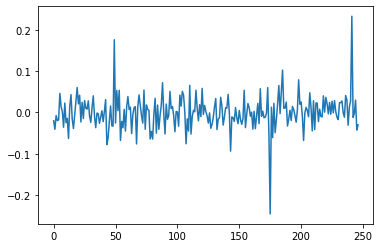
\includegraphics[width=10cm]{output.png}
\end{center}
\textbf{Summary:}
\begin{itemize}
    \item AR(1) model has the lowest value for VaR, it mainly comes from the last time y value. Since it is conditional on the $y_{t-1}$, the VaR will be affected by it. The $y_{t-1}$ here is -0.03. It is the main reason why the VaR is low under AR(1).
    \item Normal Distribution with EW has the highest value for VaR, it is because it put higher weights on the near time. According to the graph, we can find that return for META is more flexible, which leads to a higher sigma value for normal simulation. Therefore, it will increase the VaR value. (i.e. The volatility increases).
\end{itemize}
\newpage
\subsection*{Question 3. Portfolio VaR Calculation}
There, we choose Normal Monte Carlo VaR to calculate Portfolio risk separately and together. Here is the result table:\\
\begin{center}
    \begin{tabular}{ c|c|c|c|c}
     \hline
      VaR(\$) & Portfolio A & Portfolio B & Portfolio C & Total\\
     \hline
     Normal Distribution&6404&4744&4023&14751\\
     T Distribution:df = 1&11257&8562&7320&26499\\
     T Distribution:df = 100&6404&4773&4087&14853\\
     \hline
    \end{tabular}
\end{center}
\begin{center}
    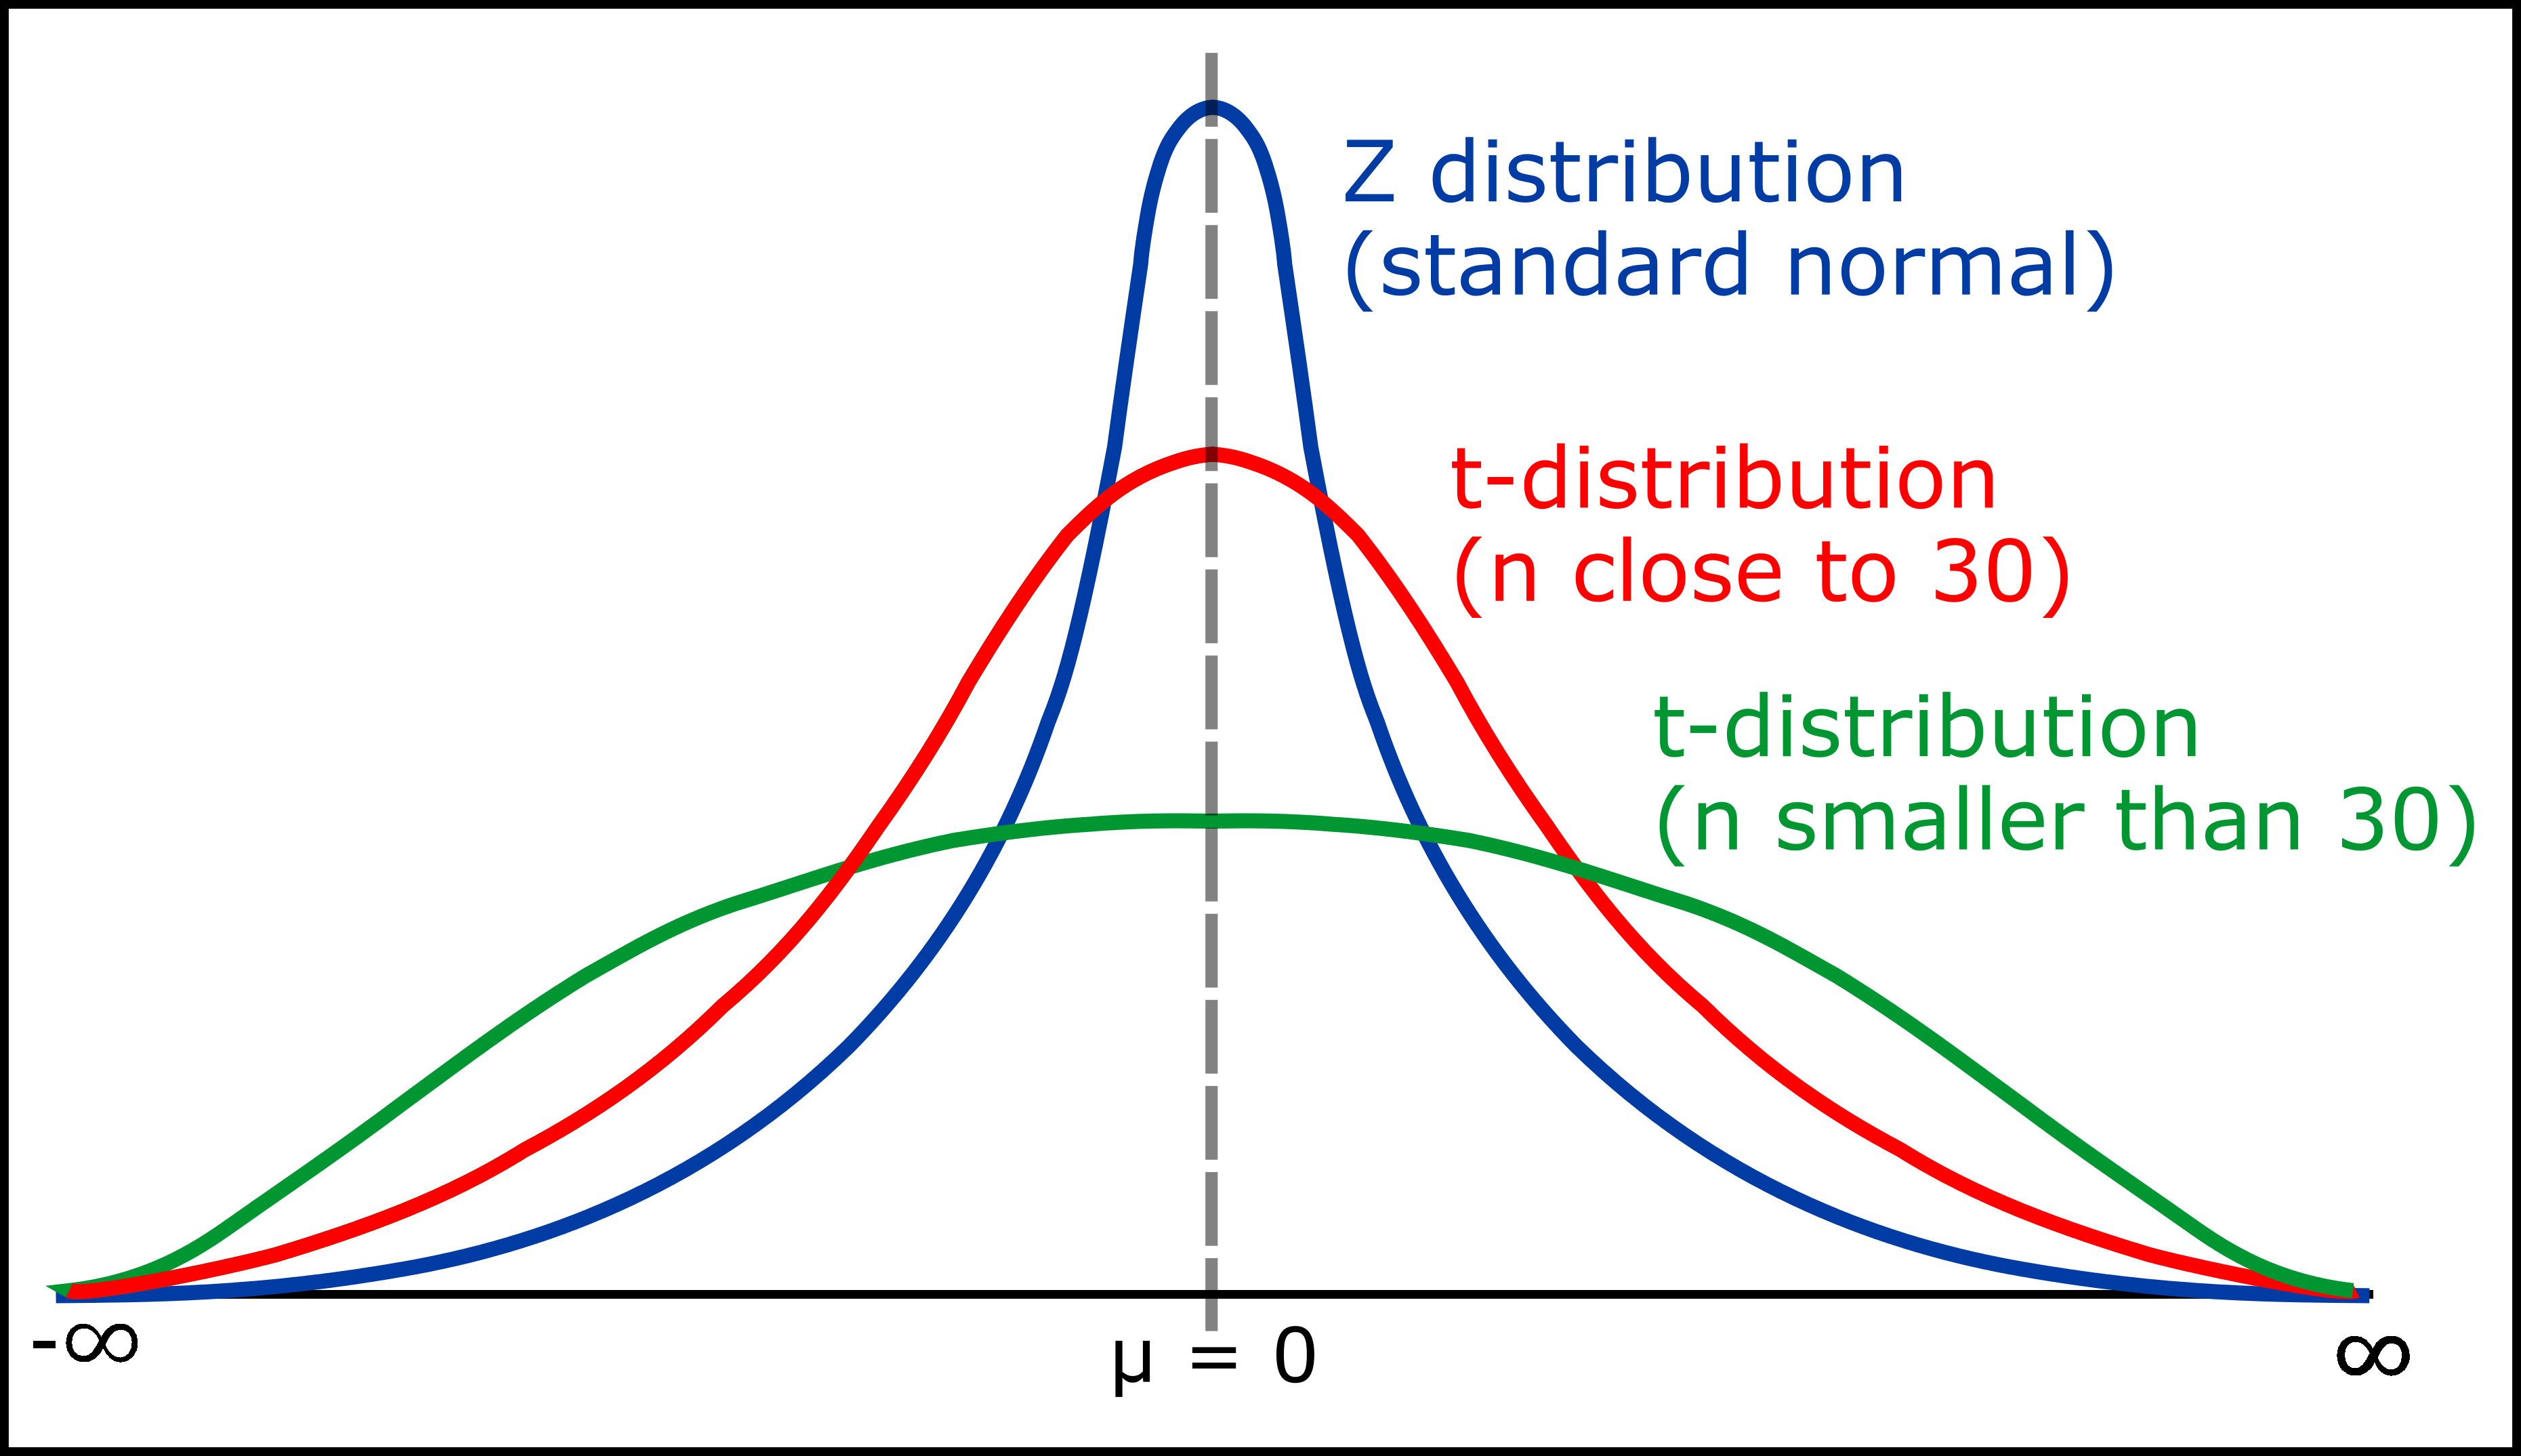
\includegraphics[width=10cm]{t_distribution.png}
\end{center}

\textbf{Summary:}
\begin{itemize}
    \item From the normal distribution simulation, we can find that the Portfolio A is high, compared with B and C. According to the table, generally VaR: A > B > C;
    \item From the T distribution simulation, we tried different settings degree of freedom settings for the VaR model, we can find that it affects the results seriously:
    \begin{itemize}
        \item According to the above graph, when degree of freedom is low, it means that we set a high probability in the tails. When the alpha is fixed, then the distance between mean and corresponding points will be higher. Finally, our VaR assessment will be higher.
        \item when degree of freedom is high, the result will approach to the result of normal distribution.
    \end{itemize}
\end{itemize}


\end{document}